\chapter{Why Do You Want to Be an Entrepreneur?}

This chapter follows Session 6, Part 1 of MIT OpenCourseWare's Nuts and Bolts of New Ventures, curated for these notes by LazyingArt LLC through Video2Book. Joseph Hadzima frames the session as a return to a personal question that had been present from the beginning: not merely how to start a venture, but whether this way of life is right for us. Bob Jones then turns that question into a disciplined inquiry. The mathematics is sparse, but it matters: a happiness heuristic, a failure-rate estimate, a hypothesis-testing loop, and a few back-of-the-envelope checks keep the chapter from becoming either startup romance or startup despair.

\section{From Venture Mechanics to Founder Fit}

The lecture begins by closing the course loop. Hadzima reminds the room that the earlier sessions have dealt mostly with factual and operational questions: whether a venture needs a corporation, how a founder finds a customer, how projections work, how negotiation and financing enter the picture. But one question was different. Is this right for you? What does entrepreneurship mean for the person who chooses it?

Jones does not answer immediately. He first asks the students what they expected from the course, what they got, and whether it had value. That exchange is not throat-clearing. It models the same customer-discovery discipline the course has been teaching. A course about customers asks its own customers what worked and what did not.

The answers also recap the course's practical orientation. Students mention distillation, negotiation, financial projections, pitches, financing sources, and the usefulness of seeing the whole process without assuming prior business training. Jones listens, draws out the distinction between high-level principle and hard execution, and then pivots: tonight's agenda is stories, the hard parts of entrepreneurship that rarely get discussed, some lessons, and a wrap-up.

So this chapter is not an inspirational appendix. It is the founder-fit chapter. The earlier lectures ask whether the venture can be built. This one asks whether we can live with what building it demands.

\section{Myths, Facts, and the Expectation Reset}

Jones begins the substance of the lecture by naming the myths. There is a popular story in which money is widely available, investors shower a brilliant idea with capital, and a boot camp can supply a magic formula for success. Some organizations half-promise that story. Jones says the course faced a moral choice: promote the myths, or tell the facts.

The first mathematical object appears exactly there.

\begin{figure}
\centering

\includegraphics[width=0.95\linewidth]{lecture_09_figure_02.png}
\caption{Hadzima's expectation heuristic as shown in the lecture.}
\end{figure}

The slide displays the compact formula
\begin{equation}
H=\frac{R}{E}.
\end{equation}
The transcript supplies the meanings of the symbols:
\begin{equation}
H=\frac{\text{reality}}{\text{expectations}},
\qquad
H=\text{happiness}.
\end{equation}
The slide itself shows the symbols and credits Hadzima; the spoken lecture gives the interpretation. We should read this as a heuristic, not as a psychological law. It is a way to say that disappointment is often caused not only by harsh reality, but by inflated expectations.

A small calculation captures the point:
\begin{align}
H &= \frac{R}{E},\\
\text{with }R\text{ fixed, increasing }E&\text{ decreases }H,\\
\text{with }R\text{ fixed, calibrating }E&\text{ stabilizes }H.
\end{align}
That is why the lecture starts with the unpleasant facts. Jones is not trying to make entrepreneurship dreary. He is trying to remove false denominators.

The facts are blunt. Entrepreneurship is hard. Most startups fail. Most investors assume the founder will probably fail, even if the founder is talented and charming. Many entrepreneurs are competing for talent, capital, and other resources, and many will not get the money.

Later Jones returns to the same point with a slide that gives the lecture's starkest quantitative claim.

\begin{figure}
\centering

\includegraphics[width=0.95\linewidth]{lecture_09_figure_05.png}
\caption{The lecture's visible failure-rate framing. The statistic is used as a lecture claim, not as a sourced universal law.}
\end{figure}

The slide's clean note form is
\begin{equation}
\text{survival after two years}\approx 10\%.
\end{equation}
Jones also states the same general claim verbally:
\begin{equation}
\text{startup failure rate}\approx 80\%\text{ to }90\%.
\end{equation}
He immediately qualifies the measurement. In the food industry, one metric is whether the product is still on the shelf two years later; other industries use other metrics. So the statistic should be treated as expectation-setting, not as a theorem about all ventures.

\begin{remark}
The point of the numbers is not precision. The point is calibration. If the expected path is easy money, then ordinary entrepreneurial reality looks like catastrophe. If the expected path includes difficulty, rejection, and revision, then the same facts can be used for learning.
\end{remark}

Jones then asks why he is talking this way. The answer is disclosure. People who enter demanding schools know they will take a beating somewhere along the way. Entrepreneurship is often promoted without the same candor. Jones wants the room to know that even smart founders fail, and that he does not know a single entrepreneur who got everything right the first time.

\section{The First Flop}

The lecture now moves from equation to story. Jones tells us about springboard diving with his fourteen-year-old daughter. The details matter because the analogy depends on the felt sequence: curiosity, fear, instruction, flop, pain, and decision.

A new diver first learns to work the board, gain height, and perform basic moves. Then comes the first real test. Jones's daughter is sent to the high board, told to turn backward with the water behind her, tuck, fall, wait for the command, come out of the tuck, find the water, and enter head first. The second time, this may seem manageable. The first time, it feels like death. She panics, fails to come out properly, and lands in a full back flop.

Jones then slows down the crossroads. She is hurt, embarrassed, and comforted. She can stop. Or she can climb back up. After a few minutes she looks at the boards, walks to the stairs, and says she is going to do it again and get it right.

The entrepreneurial analogy is direct:
\begin{equation}
\text{first serious attempt}
\longrightarrow
\text{painful flop}
\longrightarrow
\begin{cases}
\text{stop},\\
\text{try again}.
\end{cases}
\end{equation}
Jones does not say the second branch is always superior. For many people, stopping is the right decision. Entrepreneurship is not for everyone. But some people discover that the first flop did not kill them, and that discovery changes the next decision.

\subsection{Question \& Answer}

Question: After the first hard failure, why would anyone continue?

Answer: Not because failure is pleasant, and not because persistence is automatically wise. The lecture's answer is narrower. Some people reinterpret the first flop as survivable. If it is survivable, it can become information. The diver goes back up the ladder not because the pain was imaginary, but because the pain did not settle the question. Likewise, the founder who continues does not deny the failure. The founder refuses to treat one failure as the final measurement of the person.

That is the first conceptual obstacle in the lecture. If failure is identity, the story ends. If failure is experience, the next question is what the experience teaches.

\section{Failure, Rejection, and the Social Cost of Starting Up}

Jones next gives a sequence of entrepreneurial cases. Trevor starts at twenty-six with newspaper attention, a car, status, and confidence. A year later he has lost the visible symbols of success: the car is repossessed, the relationship ends, and he is living in his parents' basement while working at Radio Shack. Jones does not sanitize the humiliation. Trevor says it took years to get the taste of failure out of his mouth.

The lesson is not that humiliation is noble. The lesson is that failure was not fatal. Trevor later succeeds, but only after becoming a perpetual learner. Jones states the trait conclusion sharply:
\begin{equation}
\text{entrepreneurial survival}
\not\equiv
\text{intelligence},
\qquad
\text{entrepreneurial survival}
\not\equiv
\text{creativity}.
\end{equation}
The trait he emphasizes is adaptability:
\begin{equation}
\text{key trait}\approx \text{adaptability}.
\end{equation}

Laura's story adds the customer-discovery mechanism. She leaves a senior corporate role, assumes she is the smartest person in the room, and is shaken almost immediately by hard questions. One idea is wrong. Another consumes substantial personal money and fails. Then she realizes that the prospects are not going to use the product.

The compressed rule is one the course has been repeating:
\begin{equation}
\text{validate}
\longrightarrow
\text{talk to customers}
\longrightarrow
\text{learn whether they want it}.
\end{equation}
If customers do not want it, enthusiasm cannot force a sale.

Laura's later success comes through reaching out. She has coffee with a real-estate executive and does not initially understand the scale of his network. When he says he wants the product for all his agents, the scale becomes concrete:
\begin{equation}
\text{one useful conversation}
\longrightarrow
11{,}000\ \text{possible users}.
\end{equation}
This is not a universal distribution formula. It is a local demonstration of why private reasoning is too small. Markets are discovered through people.

Jones then turns to loneliness. The Jack-and-Jill parable is partly garbled in the transcript, but its mechanism is clear. Startup uncertainty, normal inside the venture, may sound terrifying at home. When Jack says he does not know what he is doing, Jill hears mortgage, children, savings, and risk. Jack learns that bringing self-doubt home may not be safe. But leaving it at work isolates him.

The rejection is not occasional. Customers say no. Partners say no. Investors say no. Potential employees take safer jobs. A founder who has been rewarded for intelligence and effort may enter a world where effort does not prevent repeated refusal.

Jones adds a harsher warning from another entrepreneur's story: not everyone has the founder's best interests at heart. The sidebar is direct:
\begin{itemize}
\item Do not raise money from the wrong people.
\item Protect intellectual property, especially a secret algorithm, formula, or defensible business method.
\end{itemize}

The emotional companions of this phase are anxiety, self-doubt, and imposter syndrome. A founder may present as the capable captain of the ship while privately wondering whether that is true. This is where the lecture needs a method, not another anecdote.

\section{Failure as Evidence, Not Identity}

Jones asks whether there is hope for us. His first answer is community. Ordinary friends may not understand why the founder is not simply working in a stable job. They may see the founder's choices as irrational. So Jones recommends finding a community of similarly wired people: people for whom uncertainty, ambition, repeated attempts, and bruising failures are intelligible.

Then he shifts gears. The word ``pivot'' can sound like a polite synonym for not knowing what we are doing. Jones accepts the embarrassment and then changes the frame. Scientists articulate hypotheses and test them. If a hypothesis proves wrong, they do not say that the scientist is worthless. They say it is time for the next hypothesis.

The lecture's cleanest formal structure is therefore
\begin{equation}
\text{hypothesis}
\longrightarrow
\text{test}
\longrightarrow
\text{failure/evidence}
\longrightarrow
\text{revised hypothesis}.
\end{equation}

\begin{figure}
\centering
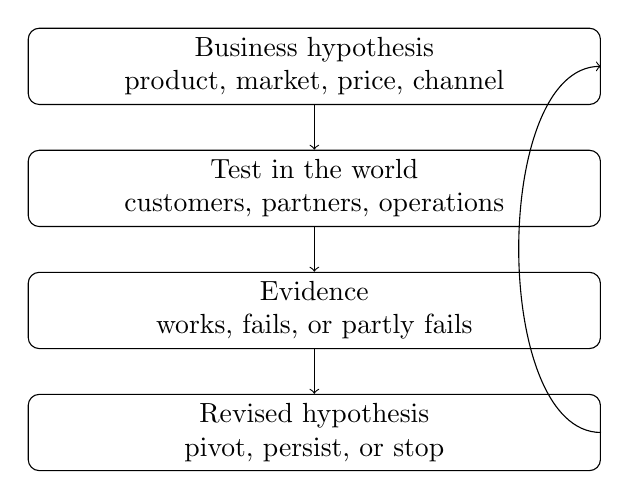
\begin{tikzpicture}[x=1cm,y=1cm]
\node[draw, rounded corners, align=center, text width=0.58\linewidth] (h) at (0,0) {Business hypothesis\\product, market, price, channel};
\node[draw, rounded corners, align=center, text width=0.58\linewidth] (t) at (0,-1.55) {Test in the world\\customers, partners, operations};
\node[draw, rounded corners, align=center, text width=0.58\linewidth] (e) at (0,-3.10) {Evidence\\works, fails, or partly fails};
\node[draw, rounded corners, align=center, text width=0.58\linewidth] (r) at (0,-4.65) {Revised hypothesis\\pivot, persist, or stop};
\draw[->] (h) -- (t);
\draw[->] (t) -- (e);
\draw[->] (e) -- (r);
\draw[->] (r.east) .. controls (2.25,-4.65) and (2.25,0) .. (h.east);
\end{tikzpicture}
\caption{A transcript-backed reconstruction of Jones's hypothesis-testing loop. It is not copied from a slide; it renders the spoken method compactly.}
\end{figure}

We can write the update rule as a cautious notation. Let \(B_n\) be the current business hypothesis at attempt \(n\), and let \(D_n\) be the evidence produced by testing it. Then
\begin{equation}
B_{n+1}=\mathrm{Revise}(B_n,D_n).
\end{equation}
This is not an algorithm that computes the next company. It is a discipline of interpretation. The practical identity to reject is
\begin{equation}
\text{failed hypothesis}=\text{failed person}.
\end{equation}
The lecture's replacement is
\begin{equation}
\text{failed hypothesis}\neq\text{failed person}.
\end{equation}

\subsection{Question \& Answer}

Question: If failure is common, how should we think about it?

Answer: We should not make it smaller than it is. Failure can cost money, time, status, confidence, and relationships. But in Jones's scientific frame, failure is also evidence. It tells us that one product, market, pricing assumption, channel, team configuration, or timing choice did not work. The useful response is not denial. The useful response is revision.

This is why the jockey analogy works. We may be a capable jockey on the wrong horse. The answer is not to insist that the horse is fine. The answer is to find a better horse.

\section{Supports: Community, Advisors, and Self-Management}

The hypothesis loop is not meant to be run alone. Jones recommends a business advisory board, and he distinguishes it sharply from a board of directors.

A board of directors represents shareholders. It has fiduciary duties. It may be empowered, and in some cases obligated, to remove the founder. That is often not the room in which to say, ``I have no idea what to do next.''

An advisory board is different. It has no fiduciary control over the company. It is a place to assemble people who know things we do not know, want the venture to succeed, and can help in narrow but crucial domains. Jones's beverage example makes the point concrete. He and a scientist friend had a \(2.5\)-ounce drink and needed a manufacturer who could bottle it below an unaffordable scale:
\begin{equation}
\text{needed production scale}<2{,}000{,}000\ \text{bottles}.
\end{equation}
Two days later, an advisor had solved the problem because the advisor knew that narrow arena.

The equity anecdote is a small cap-table lesson. Jones thought about giving each advisor one point:
\begin{equation}
\text{proposed advisor equity}=1\%.
\end{equation}
The advisors said that was too much and recommended half a point:
\begin{equation}
\text{revised advisor equity}=0.5\%.
\end{equation}
This is not a general rule that all advisors should receive \(0.5\%\). The point is that good advisors can improve not only operations but also the decisions that future investors will read as evidence of sophistication.

Jones also describes the right mix. Some advisors should be encouraging enough that we can say we fell down and hear, ``You will get up.'' But one or two should be able to give ten sensible reasons why the current plan may not work. If seven are already covered and three are new, those three are valuable.

The support structure then turns inward. Many founders believe the business must consume every hour. Jones argues that this destroys judgment, and judgment is one of the founder's scarce assets. The fixed constraint is
\begin{equation}
W=168\ \text{hours/week}.
\end{equation}
No founder gets more. Spending all of \(W\) on the company is not a proof of seriousness. It is a path to self-destruction.

Jones gives a sleep comparison from literature he encountered while working in the sleep business:
\begin{equation}
5\ \text{hours/night of sleep}
\sim
\text{cognitive impairment of three drinks}.
\end{equation}
We should keep the comparison in exactly that spirit: a lecture claim used to make the decision-quality point vivid. Frayed-out entrepreneurs make bad decisions. They may not die, as in the motorcycle analogy, but the business may.

The recommendations are plain: eat decently, exercise, walk, sleep, take care of loved ones, and do things that recharge the battery. Jones's Halloween story supplies the weight. His children remembered that he missed Halloween long after he remembered the business reason for missing it. Business issues are usually still there in the morning.

\section{Why Do It Anyway?}

After making the path difficult, Jones returns to the question that gives the lecture its title. Why would anybody do this?

He answers with several motives, and he does not reduce them to one. Some people feel they have to create something better. Some want to be their own boss badly enough to take a pay cut. Some discover that corporate life simply does not fit. Some want to improve the quality of life for others. Some want to create wealth for themselves and their families. Some love the buzz of technology or the act of building.

The service motive appears in two stories. One entrepreneur in health-care software seems, at first, to be building toward investor appeal and acquisition. But when he talks about an orphanage in Venezuela, his energy changes. Jones helps him see that the real objective may not be to grow as fast as possible toward sale. It may be to build a durable company that gives him room to support the work he cares about.

Another entrepreneur brings internet access to rural Nebraska. The business does not sound glamorous until he describes a mother who has been taking her children to a library parking lot so they can use Wi-Fi for homework. When internet access reaches her home, she can cook dinner with her children for the first time in years and return to normal work hours. That is not mythology. It is a concrete improvement in daily life.

A compact way to record the motive set is
\begin{align}
\text{entrepreneurial motive}\in
\{&
\text{autonomy},
\text{misfit with corporate life},
\text{service},
\text{wealth creation},\\
&
\text{love of building},
\text{technology excitement},
\text{creative discipline}
\}.
\end{align}
Jones's music analogy gives the last term its shape. A musician needs scales, modes, time, and framework, but also creative life inside that framework. Entrepreneurship is similar:
\begin{equation}
\text{good entrepreneurship}
\approx
\text{creativity}+\text{discipline}.
\end{equation}

\subsection{Practical Timing and Runway}

The final audience questions return the lecture to judgment. If it may take several attempts to build something valuable, how does a founder create enough runway?

Jones gives two answers. First, failed entrepreneurship does not necessarily make someone unemployable. Some companies want change agents: people who are not afraid of a blank sheet of paper and can bring creative thinking into established organizations. Second, a founder can weave in and out. Work a normal job for a while, learn, earn, calm the family situation, and later start again.

The next question is whether to keep a day job while testing the business, or to go all in. Jones argues against going all in before doing at least some market arithmetic. He refers back to the first session's back-of-the-envelope analysis:
\begin{align}
I_{\text{needed}}&=\text{income the venture must produce},\\
V_{\text{customer}}&=\text{economic value of one customer},\\
N_{\text{required}}&\approx \frac{I_{\text{needed}}}{V_{\text{customer}}}.
\end{align}
The next check is whether the market can plausibly supply that many customers:
\begin{equation}
N_{\text{reachable}}\geq N_{\text{required}}.
\end{equation}
If we have not done this sort of check, Jones says it is not the right time. If we have, it might be.

The small-step version is
\begin{equation}
\text{side test}
\longrightarrow
\text{mistakes while still paid}
\longrightarrow
\text{validation}
\longrightarrow
\text{stronger full-time pitch}.
\end{equation}
This is where passion must be governed. The right level of passion helps us work on Saturday and get back up after being knocked down. Too much passion blinds us to the obvious. Jones's rule is to deploy passion wisely.

\section{Summary}

This lecture is the personal counterpart to the operational sessions of Nuts and Bolts. The earlier material teaches incorporation, customers, projections, negotiation, and financing. This session asks whether we can live with the uncertainty, rejection, fatigue, and repeated revision that those mechanics imply.

The first tool is Hadzima's heuristic:
\[
H=\frac{R}{E}.
\]
The chapter is largely about correcting \(E\), expectations, before they distort judgment. The visible failure-rate slide and Jones's spoken estimate that eight or nine out of ten startups fail are not universal laws, but they are strong expectation-setting claims.

The most useful method is the hypothesis loop:
\[
\text{hypothesis}
\rightarrow
\text{test}
\rightarrow
\text{evidence}
\rightarrow
\text{revised hypothesis}.
\]
Failure remains painful, but it need not become identity. To survive that loop, founders need community, advisors, health, sleep, family, and a motive that survives contact with reality. Entrepreneurship has rewards for certain people, but it is not for everyone. That is not an afterthought. It is one of the course's central facts.